%%%%% Dokumentenklasse mit verschiedenen Attributen
\documentclass[a4paper, bibtotocnumbered,liststotoc,12pt,abstracton]{scrartcl}

%%%%% Betriebssystemabh�ngige Eingabedekodierung
\usepackage[T1]{fontenc}
\usepackage[latin1]{inputenc} %% f�r Windows

%%% Python code
\usepackage{listings}             % Include the listings-package
\lstset{language=Python}          % Set your language (you can change the language for each code-block optionally)


%%%%% \usepackage[applemac]{inputenc} %% f�r Mac
\usepackage[ngerman, english]{babel}

%%%% Arial
%\usepackage{uarial}
%\renewcommand{\familydefault}{\sfdefault}
%\usepackage{blindtext}

%%%%% Zeilenabstand
\usepackage{setspace}
\onehalfspacing %anderthalbzeilig

%%%%% Mathematik und Symbole
\usepackage{amsmath}
\usepackage{amssymb}
\usepackage{amsthm}

%%%%% Seitenr�nder und Ausrichtung
\usepackage[paper=a4paper,left=30mm,right=25mm,top=25mm,bottom=35mm]{geometry} %define margins..
\geometry{a4paper} % hier auch m�glich 'letter' oder 'a5paper' ... etc.
\usepackage{lmodern}
\usepackage{verbatim}
\setkomafont{sectioning}{\rmfamily\bfseries\boldmath}
\usepackage[usenames,dvipsnames]{color}


%%%%% �berschriften
%\pagestyle{headings} %F�gt �berschrift �ber jeder Seite ein

\usepackage{overcite}

%%%%% Tabellen und Grafiken
\usepackage{booktabs}
\usepackage{tabularx}
\usepackage{array}
\usepackage{graphicx}
\usepackage{rotating}
\usepackage{xtab}
\usepackage{float}

%%%%% Sonstiges

%%%%% Umgebungen f�r S�tze, Propositionen,...
\newtheorem{satz}{Satz}
\newtheorem{prop}{Proposition}
\newtheorem*{beweis}{Beweis}

%%%%%%%%%%%%%%%%%%%%%%%%%%%%%%%%%%%%%%%%%%%%%%%%%%%%%%%%%%%%%%%%%%%%%%%
%%%%% BEGIN DOCUMENT %%%%%%%%%%%%%%%%%%%%%%%%%%%%%%%%%%%%%%%%%%%%%%%%%%%%%%%
\begin{document}
\selectlanguage{english}

%%%%%%%%%%%%%%%%%%%%%%%%%%%%%%%%%%%%%%%%%%%%%%%%%%%%%%%%%%%%%%%%%%%%%%%
%% TITLE PAGE %%%%%%%%%%%%%%%%%%%%%%%%%%%%%%%%%%%%%%%%%%%%%%%%%%%%%%%%%%%%%%
\selectlanguage{ngerman}
\begin{titlepage}
\large{Timo Meiendresch}
 \vspace{\fill}
\begin{center}
\Huge{Recurrent Neural Networks for Time Series Forecasting}\\
\large{}
\end{center}
 \vspace{\fill}
\large{Capstone Project} \\
\large{Machine Learning Engineer Nanodegree (Udacity)}\\
\vspace{\fill}\\ Cologne 2019\\
%Cologne
\end{titlepage}
\selectlanguage{english}
%%%% Inhalts-, Abbildungs- und Tabellenverzeichnis
\tableofcontents %f�gt ein Inhaltsverzeichnis ein
\listoffigures % f�gt ein Abbildungsverzeichnis ein 
\listoftables % f�gt ein Tabellenverzeichnis ein %\newpage % Seitenumbruch %%%%%%%%%%%%%%%%%%%%%%%%%%%%% Hauptteil %%%%%%%%%%%%%%%%%%%%%%%%%%%%%%%
\newpage
\begin{abstract} 
The year is 2019 A.D. Quantitative research is entirely occupied by Machine Learning (ML). Well, not entirely... One small group of indomitable forecasters still holds out against the invaders. And life is not easy for the ML evangelists who garrison the fortified camps of quantitative research. 
\end{abstract}


\section{Introduction}
% Importance of time series forecasting
It is widely perceived, that time series forecasting is an essential tool in business, economics, and many other disciplines. The ability to accurately infer future variables given historic data is of huge value to decision makers. 

% Surge of ML methods 
In recent years, \textbf{Machine Learning (ML)} methods had huge success in many areas of quantitative research. Prominent examples include classification tasks, image processing, or text analysis. ML took many fields by storm and it seems that many quantitative discipline can benefit from giving in to the AI wave.

% Contrast to time series forecasting
And yet, in the area of time series forceasting, machine learning methods are rarely considered. In this area they have a history of inferior performance compared to simpler, traditional methods. Particular examples of these traditional methods include the \textbf{Autoregressive Integrated Moving-Average (ARIMA)} and \textbf{Exponential Smoothing (ES)} methods. 

% Perception
Until recently, a widely shared perception among researchers was that complex methods for time series forecasting in general, such as neural networks, were not performing better than traditional ones (e.g. Hyndman, 2019). Among others, Makridakis et al. (2018) noted that there is only very limited scientific evidence which suggests that artificial neural networks may be a useful tool for time series forecasting. 


\subsubsection*{Paradigm Shift}
But, advances in recent years start to challenge this notion. For example, the winner of the most recent version of the M4 time series competition (Makridakis et al., 2019) was an elaborate hybrid of a \textbf{recurrent neural network (RNN)} architecture with ES methods (Smyl, 2019). Measured on a diverse dataset of 100,000 univariate time series from six domains and frequencies, this method outperformed traditional ones, pure statistical combinations as well as ML-based combination methods. The results of the competition showed the potential of recurrent networks for time series forecasting, leading to a surge of algorithms in this area. It also showed that RNN could successfully be trained on highly diverse data. Commonly, RNN methods for time series foreasting are applied to a large set of homogeneous data.  

\subsubsection*{Local vs. global methods}
Moreover, the M4 competiton highlights an ongoing paradigm shift in the forecasting community. Traditional methods like ARIMA and ES are applied to individual series. These \textbf{local} methods estimate a number of parameters within a model space that is restricted by the respective structure of the model. Because these approaches rely on an explicit model structure they are referred to as \textbf{model-based} (Wang et al., 2019). Each series is modeled and trained independent of other series in the data set. Hence, the individual model is independent of the total number of series in the dataset as well as its characteristics in terms of similarity.

Also, with the emergence and availability of large sets of data a new forecasting problem emerges. It is becoming increasingly necessary to implement large-scale forecasting systems that simultaneously predict many related series. Examples include predictions of product sales in online retailers, household energy consumption, or web traffic. In contrast to local models, \textbf{global} methods enable the use of \textbf{cross-series learning}, i.e. the training process uses all available time series and yields a representation of the entire data set. In theory, RNN-based methods are therefore able to learn across individual series and extract general patterns of the data as well as learn dependency relationships between the individual series which may improve forecasting accuracy. 

In the aftermath of the M4 competition, various methods have been published that are based on the idea of cross-series learning, often combining local with global methods. If and under which conditions these models actually perform better than local ones is a relatively new question into which very little empirical research has so far been done. 

In theory, RNN should be able to work as a universal function approximator if it is only powerful enough. In practice however, the learnability of RNNs is limited. A typical problem is that they do not converge during training. They are considered to be difficult to train. This is an important factor for practitioner's as training a powerful network on such a huge amount of data is computationally expensive. 

Hence, it seems that there are two main properties of the underlying data that should be considered in the following analysis: 

\begin{itemize}
\item[] Property 1 - Total number of individual time series in the underlying data set. How many series are in the dataset?
\item[] Property 2 - Similarity of the individual time series in the data set. How diverse are the series?
\end{itemize}

This leads to two hypothetically important caveats regarding the dataset which influence the performance. The total number of time series in the dataset as well as how diverse the series are with respect to each other.

Often these methods lack rigorous comparison with previous methods and known data sets. This capstone project investigates the performance of three RNN-based methods developed in the last two years, namely: 

\begin{itemize}
\item \textbf{Deep Autoregressive Recurrent Neural Networks (DeepAR)} - Wang et al. (2019)
\item \textbf{Deep State Space Models (DeepState)} - Rangapuram et al. (2018)
\item \textbf{Deep Neural Network Factor Models (DeepFactor)} - Wange et al. (2019)
\end{itemize}

To evaluate these models I will apply them to the Hourly, Daily, Weekly and Monthly data of the M4 competition using the same metrics that were used in the competiton. Hence, a variety of benchmarks is available for comparison. 

% Heterogeneous data vs. Homogeneous data?
Note that these methods are designed to be applied to large sets of related data. In contrast, the M4 data set is a diverse dataset from many domains and frequencies.

To the best of my knowledge, no comparison of these algorithms to the M4 benchmarks has been published yet. The primary contribution of this paper is to evaluate these algorithms on the well studied M4 data and compare the results to known benchmarks. 

The rest of the paper is organized as follows. I first discuss ... in Section ....

\section{Definition}
\subsubsection*{Project Overview}
% High-level overview of the project
% Background information such as the problem domain
% Project origin
% related data sets or input data given
This project compares three RNN-based algorithms for time series forecasting to the well studied M4 data and its benchmarks, including modern and traditional methods. The data include the original M4 data for hourly, daily, weekly, and monthly frequencies. 

\subsubsection*{Problem Statement}
% Clearly defined
% Strategy for solving the problem
% Discussion of expected solution
Main goal of this paper is to evaluate the performance of the three algorithms DeepAR, DeepState, and DeepFactor with respect to traditional and state-of-the art methods. The main question is to give a quick assessment of their competitiveness starting from their default hyperparameters. The accuracy is assessed using the same metrics that were used during the competition.

\subsubsection*{Metrics}
The performance of the methods is evaluated using the same two measures that were used in the M4 competition to evaluate the forecast accuracy. Forecast measures are still a highly active area of research and there is no consensus on which one is considered to be the best one. Hence, two widely used \textbf{scale-independent errors} have been used in the competition. Scale-independent means they are independent of the unit of the time series. Because the competition evaluates accuracy across highly diverse time series, a scale-independent measure is required. The two measures are:
\begin{itemize}
\item \textbf{Symmetric mean absolute percentage error (sMAPE)}
\item \textbf{Mean absolute scaled error (MASE)}
\end{itemize}
The \textbf{sMAPE} belongs to the class of percentage errors. While this makes the measure unit-free it has the disadvantage of being infinite/undefined if the target variable is zero for any $t$ in the period of interest, and is highly skewed towards extreme values if the target variable is close to zero. The measure is defined as 
\begin{align*}
sMAPE = \frac{1}{h} \sum_{t=1}^h \frac{2 \,|Y_t-\hat{Y}_t |}{|Y_t| + |\hat{Y}_t|}
\end{align*}
where $Y_t$ is the post-sample value, $\hat{Y}_t$ the estimated forecast, and $h$ the forecasting horizon.

Alternatively, Hyndman and Koehler (2006) propose the scaled error measure \textbf{MASE} when comparing forecast accuracy across series with different units. In this case the absolute error is scaled using the \textbf{Mean Absolute Error (MAE)} from a simple forecast method (either naive or seasonal naive method). The method is defined for seasonal in the following way: 
\begin{align*}
MASE = \frac{1}{h} \, \frac{ \sum_{t=1}^h |Y_t - \hat{Y}_t| }{ \frac{1}{n-m} \sum_{t=m+1}^n |Y_t - Y_{t-m}|}
\end{align*}
where $m$ indicates the seasonality of the series. In case of non-seasonal data $m=1$, $Y_t - Y_{t-m}$ simplifies to $Y_t - Y_{t-1}$ being the naive forecast error. The naive forecast predicts the next value to be equal to the last value $\hat{Y}_{t+1} = Y_t$. This yields the non-seasonal version of the MASE as 
\begin{align*}
MASE = \frac{1}{h} \, \frac{ \sum_{t=1}^h |Y_t - \hat{Y}_t| }{ \frac{1}{n-m} \sum_{t=m+1}^n |Y_t - Y_{t-m}|}
\end{align*}
In addition to evaluating point forecasts, the performances of prediction intervals has also been part of the competition. Specifically, the \textbf{Mean Scaled Interval Score (MSIS)} has been used for this. Moreover, other widely used measures for evaluating forecast accuracy include the normalized sum of quantile losses for quantiles $p \in {0.5, 0.9}$. As these were the preferred measures in some of the mentioned papers I have decided to include them for reference together with the MSIS. However, there is high correlation between the two forecast measures and MSIS as well as there are some methods that do not give quantile losses. Therefore, I will not discuss these results explicitly.


\section{Analysis}
\subsubsection*{Data Exploration}
The dataset consists of 100,000 univariate time series from six domains, divided in six different frequencies. 
\begin{table}[h]
\label{fig_m4_overview}
\centering
\textbf{M4 Data  - Overview}\par\medskip
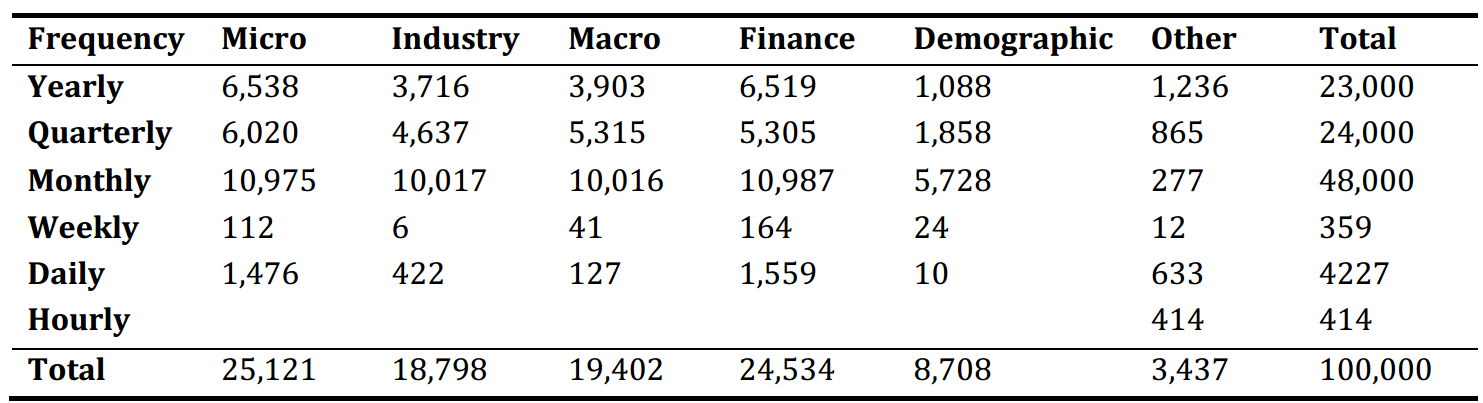
\includegraphics[scale=.58]{../images/M4_data_overview.png} 
\caption{M4 data by domains and frequencies.}
\end{table}
They were chosen from a database of more than 900,000 time series. One time series consists of a date and a respective observation for that date where the frequency determines the space between two observations. In this dataset, all frequencies are equidistant which means that the time between two observations is constant. 

Common characteristics include seasonal patterns, cyclic behavior, as well as trends that the model has to capture. Given the behavior of the series, the method has to extrapolate the series into the future. The number of future observations that have to be forecasted were given by the instructions of the competitions:
\begin{table}[h]
\label{tab_horizons}
\centering
\textbf{M4 Data - Forecast Horizons}\par\medskip
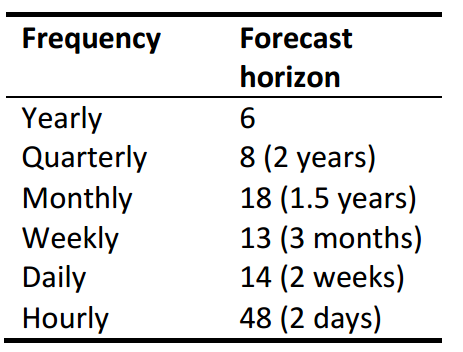
\includegraphics[scale=0.6]{../images/M4_data_forecast_horizon.png} 
\caption{Forecast horizons by frequency of the data.}
\end{table}
A key challenge for the prediction method is the high diversity of the data. Some data exhibit cyclical behavior, whereas other series have up- or downward trends, or varying seasonal patterns. Capturing the behavior accurately for all series is the goal of time series forecasting. 

\subsubsection*{Exploratory Visualization}
The dataset is highly diverse with respect to domain and frequency. For each series there exist a train data as well as extended test data. The test data consists of the train data and the additional, previously unknown observations that have to be forecasted. A randomly chosen example series from the hourly M4 dataset is depicted below: 
\begin{figure}[h]
\label{series338}
\centering
\textbf{M4 Hourly - Series \#338}\par\medskip
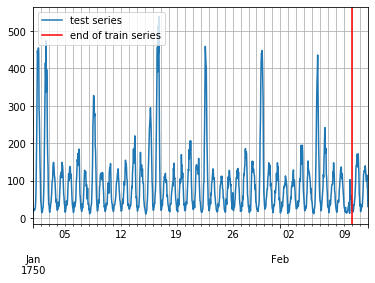
\includegraphics[scale=0.75]{../images/train_test_plot_m4_hourly338.png} 
\caption{Example series over time. The vertical red line indicates the break between train and test dataset.}
\end{figure}

\subsubsection*{Algorithms and Techniques}
In this paper I will compare three RNN-based algorithms to the results of the M4 competition. 

The first of the three algorithms is the  \textbf{Deep Autoregressive Recurrent Neural Network (DeepAR)} method, introduced by Salinas et al. (2017). It is the only built-in time series prediction algorithm in the AWS SageMaker which enables machine learning in the cloud. DeepAR uses autoregressive features that are used as the inputs to a recurrent neural network. The RNN uses LSTM cells as default but can also be changed to GRU cells. Previous observations are taken in as inputs which makes this algorithm autoregressive. Which autoregressive features are included depends on the frequency of the data. 

Rangapuram et al. (2018) introduced \textbf{Deep State Space Models (DeepState)}. DeepState combines state space models (SSM) with a recurrent neural network architecture that calculates the optimal parameters for the SSM. The SSM is applied locally to the individual time series. The parameters are determined by a RNN which is trained jointly on all available series.

Furthermore, I included the \textbf{Deep Factor} model by Wang et al. (2019). This hybrid algorithm uses local methods that are specific to each time series in the dataset as well as a global representation trained on the entire data. For now, the only local method that is available is a smaller RNN. Hence, the model combines a local RNN with a global RNN (DeepFactor-RNN or DF-RNN in the following). Main differences between the algorithms: 
\begin{itemize}
\item \textbf{DeepAR} - Pure RNN that uses autoregressive features as inputs. 
\item \textbf{DeepState} - Uses RNN to determine the best parameters of the individual SSM
\item \textbf{DF-RNN} - Hybrid of a local RNN (individual time series) that is combined with a global RNN (all time series)
\end{itemize}
The training process for all three algorithms uses a fixed window approach. During training, batches of time series windows in the training data are fed to the algorithm. Each time series window is a sliced version of the entire series starting at different points of the series and has length of the training range plus prediction range. Here, the prediction range corresponds to the forecasting horizon of our model. 


\subsubsection*{Benchmark}
In addition to providing a rich dataset across frequencies and domains, a key contribution of the M4 competition is the provision of a rich set of benchmark methods. Not only the metrics of the competition winners but also results for commonly used methods, in particular ARIMA and ES, are provided in Hyndman et al. (2019). In the discussion of the results I will focus on the relative performance of the RNN-based methods with respect to: 
\begin{enumerate}
\item seasonally adjusted naive predictions (Naive2)
\item traditional methods (ARIMA and ES)
\item overall winning method of Smyl (2019), runner-up by Montero-Manso et al. (2019) as well as the winning method of the respective frequency 
\end{enumerate}


\section{Methodology}
\subsubsection*{Data Preprocesing}
The data has to be prepared in a certain way to be valid inputs to the algorithms. Namely, it is required to be in json lines like format which in python is essentially a dictionary of dictionaries. Inputs must contain at least the following keys with respective content: 

\begin{itemize}
\item `start` - Timestamp with the format YYYY-MM-DD HH:MM:SS and the respective frequency of the data
\item `target` - An array of floats or integers that represents the target series of interest. 
\end{itemize}
An example input file takes the form

\begin{lstlisting}[frame=single]
# get first entry in dataset.train
entry = list(dataset.train)[0]

# first entry
entry
>>> {'start': Timestamp('1750-01-01 00:00:00', freq='H'),
 'target': array([605., 586., 586., ..., 521.], dtype=float32)
\end{lstlisting}

Additional fields are optional. One important field 

\subsubsection*{Implementation}

\subsubsection*{Refinement}


\section{Results}

\subsubsection*{Model Evaluation and Validation}

\subsubsection*{Justification}


%Conclusion (0.5-1 page)

%%%%%%%%%%%%%%%%%%%%%%%%%%%%%%%%%%%%%%%%%%%%%%%%%%%%%%%%%%%%%%%%%%%%%%%%%%%%%%%%%%%%%%%%%%%%%%%%%%%
%%%%%%%%%%%%%%%%%%%%%%%%%%%%%%%%%%%%%%%%%%%%%%%%%%%%%%%%%%%%%%%%%%%%%%%%%%%%%%%%%%%%%%%%%%%%%%%%%%%


%%%%%%%%%%%%%%%%%%%%%%%%%%%%%%%%%%%%%%%%%%%%%%%%%%%%%%%%%%%%%%%%%%%%%%%%%%%%%%%%%%%%%%%%%%%%%%%%%%%
%%%%%%%%%%%%%%%%%%%%%%%%%%%%%%%%%%%%%%%%%%%%%%%%%%%%%%%%%%%%%%%%%%%%%%%%%%%%%%%%%%%%%%%%%%%%%%%%%%%


%%%%%%%%%%%%%%%%%%%%%%%%%%%%%%%%%%%%%%%%%%%%%%%%%%%%%%%%%%%%%%%%%%%%%%%
%% Anhang %%%%%%%%%%%%%%%%%%%%%%%%%%%%%%%%%%%%%%%%%%%%%%%%%%%%%%%%%%%%%%
%%%%%%%%%%%%%%%%%%%%%%%%%%%%%%%%%%%%%%%%%%%%%%%%%%%%%%%%%%%%%%%%%%%%%%%
%% LITERATURE %%%%%%%%%%%%%%%%%%%%%%%%%%%%%%%%%%%%%%%%%%%%%%%%%%%%%%%%%%%%%

% View complete list of literature in database
%\nocite*

% List of references
\newpage
%\bibliography{dateiname.bib}
\bibliographystyle{plain}
 \begin{thebibliography}{------}
%alphabetisch sortieren

	\bibitem{Hyndman2019}
Hyndman, Rob J. "A brief history of forecasting competitions." \textit{International Journal of Forecasting (2019)}.
	
	\bibitem{HK2006}
Hyndman, Rob J., and Anne B. Koehler. "Another look at measures of forecast accuracy." \textit{International journal of forecasting 22.4 (2006): 679-688.}

	\bibitem{RSG+2018}
Rangapuram, Syama Sundar, et al. "Deep state space models for time series forecasting." \textit{Advances in Neural Information Processing Systems}. 2018.

	\bibitem{SFG2017}
Salinas, David, Valentin Flunkert, and Jan Gasthaus. "DeepAR: Probabilistic forecasting with autoregressive recurrent networks." \textit{arXiv preprint arXiv:1704.04110 (2017).}

	\bibitem{Smyl2019}
Smyl, Slawek. "A hybrid method of exponential smoothing and recurrent neural networks for time series forecasting." \textit{International Journal of Forecasting (2019).}

	\bibitem{SE+2019}
Spiliotis, Evangelos, et al. "Are forecasting competitions data representative of the reality?." \textit{International Journal of Forecasting (2019).}

	\bibitem{MEV2018}
Makridakis, Spyros, Evangelos Spiliotis, and Vassilios Assimakopoulos. "Statistical and Machine Learning forecasting methods: Concerns and ways forward." \textit{PloS one 13.3 (2018):
e0194889.}

	\bibitem{MEV2019}
Makridakis, Spyros, Evangelos Spiliotis, and Vassilios Assimakopoulos. "The M4 competition: 100,000 time series and 61 forecasting methods." \textit{International Journal of Forecasting
(2019).}

	\bibitem{W+2019}
Wang, Yuyang, et al. "Deep Factors for Forecasting." \textit{arXiv preprint arXiv:1905.12417 (2019).}

 \end{thebibliography}


%%%%%%%%%%%%%%%%%%%%%%%%%%%%%%%%%%%%%%%%%%%%%%%%%%%%%%%%%%%%%%%%%%%%%%%
%% EIDESSTATTLICHE ERKL�RUNG  %%%%%%%%%%%%%%%%%%%%%%%%%%%%%%%%%%%%%%%%%
%\newpage
%\selectlanguage{ngerman}
%\section*{Eidesstattliche Erkl�rung}
%Hiermit versichere ich, dass ich die vorliegende Arbeit selbstst�ndig und ohne die Benutzung anderer als der angegebenen Hilfsmittel angefertigt habe. Alle Stellen, die w�rtlich oder sinngem�� aus ver�ffentlichten und nicht ver�ffentlichten Schriften entnommen wurden, sind als solche kenntlich gemacht.\\
%\\
%K�ln, den \today
%\\
%Unterschrift
%\selectlanguage{english}
\end{document}
